% -*- root: ../../thesis.tex -*-

% empty page style for toc
% http://tex.stackexchange.com/questions/2995/removing-page-number-from-toc
\addtocontents{toc}{\protect\thispagestyle{empty}}

\chapter[webchem: An R Package to Retrieve Chemical Information]{webchem: An R Package to Retrieve Chemical Information from the Web}
\addthumb{\thechapter}{\Huge\thechapter}{white}{gray}
\label{sec:webchem}  

\begin{sloppypar}
\bigskip
\underline{Eduard Szöcs\textsuperscript{a}} \& Ralf B. Schäfer\textsuperscript{a}

\bigskip
\small
\noindent 
\textsuperscript{a}Institute for Environmental Sciences, University Koblenz-Landau, Landau, Germany 

\bigskip 
\normalsize
\noindent
Accepted in \emph{Journal of Statistical Software}, 2016.

\end{sloppypar}
\cleardoublepage


%% ----------------------------------------------------------------------------
\section{Abstract}
A wide range of chemical information is freely available online, including identifiers, experimental and predicted chemical properties.
However, these data are scattered over various data sources and not easily accessible to researchers.
Manual searching and downloading of such data is time-consuming and error-prone.  
We developed the open-source R package webchem that allows users to automatically query chemical data from currently 11 web sources. 
These cover a broad spectrum of information.
The data are automatically imported into an R object and can directly be used in subsequent analyses.
webchem enables easy, structured and reproducible data retrieval and usage from publicly available web sources.
In addition, it facilitates data cleaning, identification and reporting of substances.
Consequently, it reduces the time researchers need to spend on chemical data compilation.

\section[Introduction]{Introduction}
Before each statistical analysis, data cleaning is often required to ensure good data quality.
Data cleaning is the process of detecting errors and inconsistencies in data sets \citep{Chapman_2005}.
In practice, the data cleaning step is often more time consuming than the subsequent statistical analysis, particularly, when the analysis relies on the joining of multiple data sources.

When dealing with chemical data sets (e.g.\ environmental monitoring data, toxicological data), a first step is often to validate the names of chemicals or to link them to unique codes that simplify subsequent querying and appending of compound-related physico-chemical or toxicological information.
Several web sources provide chemical names or link them to unique codes (see also section \emph{Data sources} below).
However, manual searching for each compound, often through a graphical web interface, is tedious, error-prone and not reproducible \citep{Peng_2009}.

To simplify, robustify and automate this task, i.e.\ to search and retrieve chemical information from the web, we created the webchem package for the free and open source R language \citep{r_2015, Wehrens_2011}.
R is one of the most widely used software environments for data cleaning, analysing and visualising data, and supports full reproducibility of each step \citep{Marwick_2016}.

In the following, we describe the basic functionality of the package and demonstrate with a few use cases how to clean and retrieve new data with webchem.


\section[Implementation and design details]{Implementation and design details}
The webchem package is written entirely in R and available under a MIT license.
The development repository is hosted on \citet{github} and a stable version is released on the official R repository \citep{cran}.
webchem is part of the rOpenSci project \citep{boettiger2015building}, which aims at fully reproducible data analysis.

webchem follows best practices for scientific software \citep{wilson_best_2014, poisot_best_2015}, namely: (i) a public available repository with easy collaboration and an issue tracker (via GitHub), (ii) a non-restrictive license, version control (git), (iii) an elaborate test-suite covering more than 90\% of the relevant lines of code (currently approximately 1500 lines, using testthat \citep{wickham_testthat:_2011}), (iv) continuous integration (via \citet{travis-ci} and \citet{appveyor}; testing on Linux \& Windows with current and development R versions), (v) in-source documentation (using roxygen2 \citep{wickham_roxygen2:_2015}) and (vi) compliance with a style guide \citep{wickham_advanced_2015}.

webchem builds on top of the following R packages:
RCurl \citep{lang_rcurl:_2015} and httr \citep{wickham_httr} for data transfer,
stringr \citep{wickham_stringr:_2015} for string handling,
xml2 \citep{wickham_xml2} and rvest \citep{wickham_rvest} for parsing HTML and XML,
jsonlite \citep{ooms_jsonlite_2014} for parsing JSON,
rcdk \citep{guha_rcdk} for parsing SMILES.
For parsing molfiles we use a lightweight implementation of \citet{Grabner_Varmuza_Dehmer_2012}.

Some data sources provide application programming interfaces (API).
Web APIs define functions that allow accessing services and data via http and return data in a specific way.
webchem uses the API of a data source provider, where available.
For sources where an API is lacking, data is directly searched and extracted from the web pages, analogous to manual interaction with a website.

Only few design decisions have been made:
Each function name has a prefix and suffix separated by an underscore \citep{Chamberlain_Szocs_2013}.
They follow the format of source\_function, e.g.\ cs\_compinfo uses ChemSpider as source (see next section) to retrieve compound information.
Some functions require querying first a unique identifier from the data source and then use this identifier to query further information.
The prefix get is used to denote these functions, e.g.\ get\_csid to retrieve the identifier used in ChemSpider.

webchem is friendly to the resources of data providers. 
Between each request there is a time-out of 0.3 to 2 seconds depending on the data source. 
Therefore, processing of larger data sets can take some time, but still represents a major improvement compared to manual lookup.
We provide a link to the \emph{Terms of Use} of data providers in the documentation of each function and we encourage the users to read these before using webchem.
Moreover, all functions return an URL of the source, which can be used for \mbox{(micro-)attribution}.


\section[Data sources]{Data sources}
The backbone of webchem are data sources providing their data and functionality to the public.
Currently, data can be retrieved from 11 sources.
These cover a broad spectrum of available data, like identifiers, experimental and predicted properties and regulatory information (Figure~\ref{fig:fig1}, a detailed overview of all sources is included as supplement):

\clearpage

\begin{description}
  \item[NIH Chemical Identifier Resolver (CIR)]{A web service that converts \\from and to various chemical identifiers \citep{cir}.}
  \item[Chemical Translation Service (CTS)]{A web service that converts from and to various chemical identifiers \citep{wohlgemuth_haldiya_willighagen_kind_fiehn_2010}.}
  \item[ETOX]{Information System Ecotoxicology and Environmental Quality Targets by the German Federal Environmental Agency. Provides basic identifiers, synonyms, ecotoxicological data and quality targets for different countries \citep{etox}.}
  \item[PAN Pesticide Database]{Information on pesticides - provides basic identifiers, ecotoxicological data and chemical properties \citep{pan}.}
  \item[SRC Physprop]{Contains physical properties for over 41,000 chemicals.
  Physical properties collected from a wide variety of sources including experimental and modeled values\citep{physprop}.}
  \item[PubChem]{PubChem is a public repository for information on chemical substances, providing identifiers, properties and synonyms \citep{kim2016}.
  We use an interface to the PUG-REST web service \citep{Kim_Thiessen_Bolton_Bryant_2015}.}
  \item[Wikidata]{Wikipedia contains information for over 15,000 chemicals \citep{Ertl_Patiny_Sander_Rufener_Zasso_2015, wiki}. Currently webchem can only query chemical identifiers.}
  \item[Compendium of Pesticide Common Names]{The compendium provides information on pesticide common names, identifiers and classification \citep{wood}.}
  \item[ChemID\emph{plus}] {is a large web-based database provided by the National Library of Medi\-cine (NLM). It provides identifiers, synonyms, toxicological data and chemical properties \citep{tomasulo2002}.}
  \item[ChemSpider]{is a free chemical structure database providing access to over 40 million structures. It provides identifiers, properties and can also be used to convert identifiers \citep{pence_chemspider:_2010}.}
  \item[OPSIN]{The Open Parser for Systematic IUPAC nomenclature is a chemical name interpreter and provides InChI and SMILES identifiers \citep{lowe_corbett_murray-rust_glen_2011}.}
\end{description}

Though the data sources exhibit some overlap in the provided information, each has been selected because it also provides unique information and we encourage the interested reader to consult the related source for details. 
However, we provide a brief overview in the Supporting Information.

\begin{figure}[H]
  \centering
  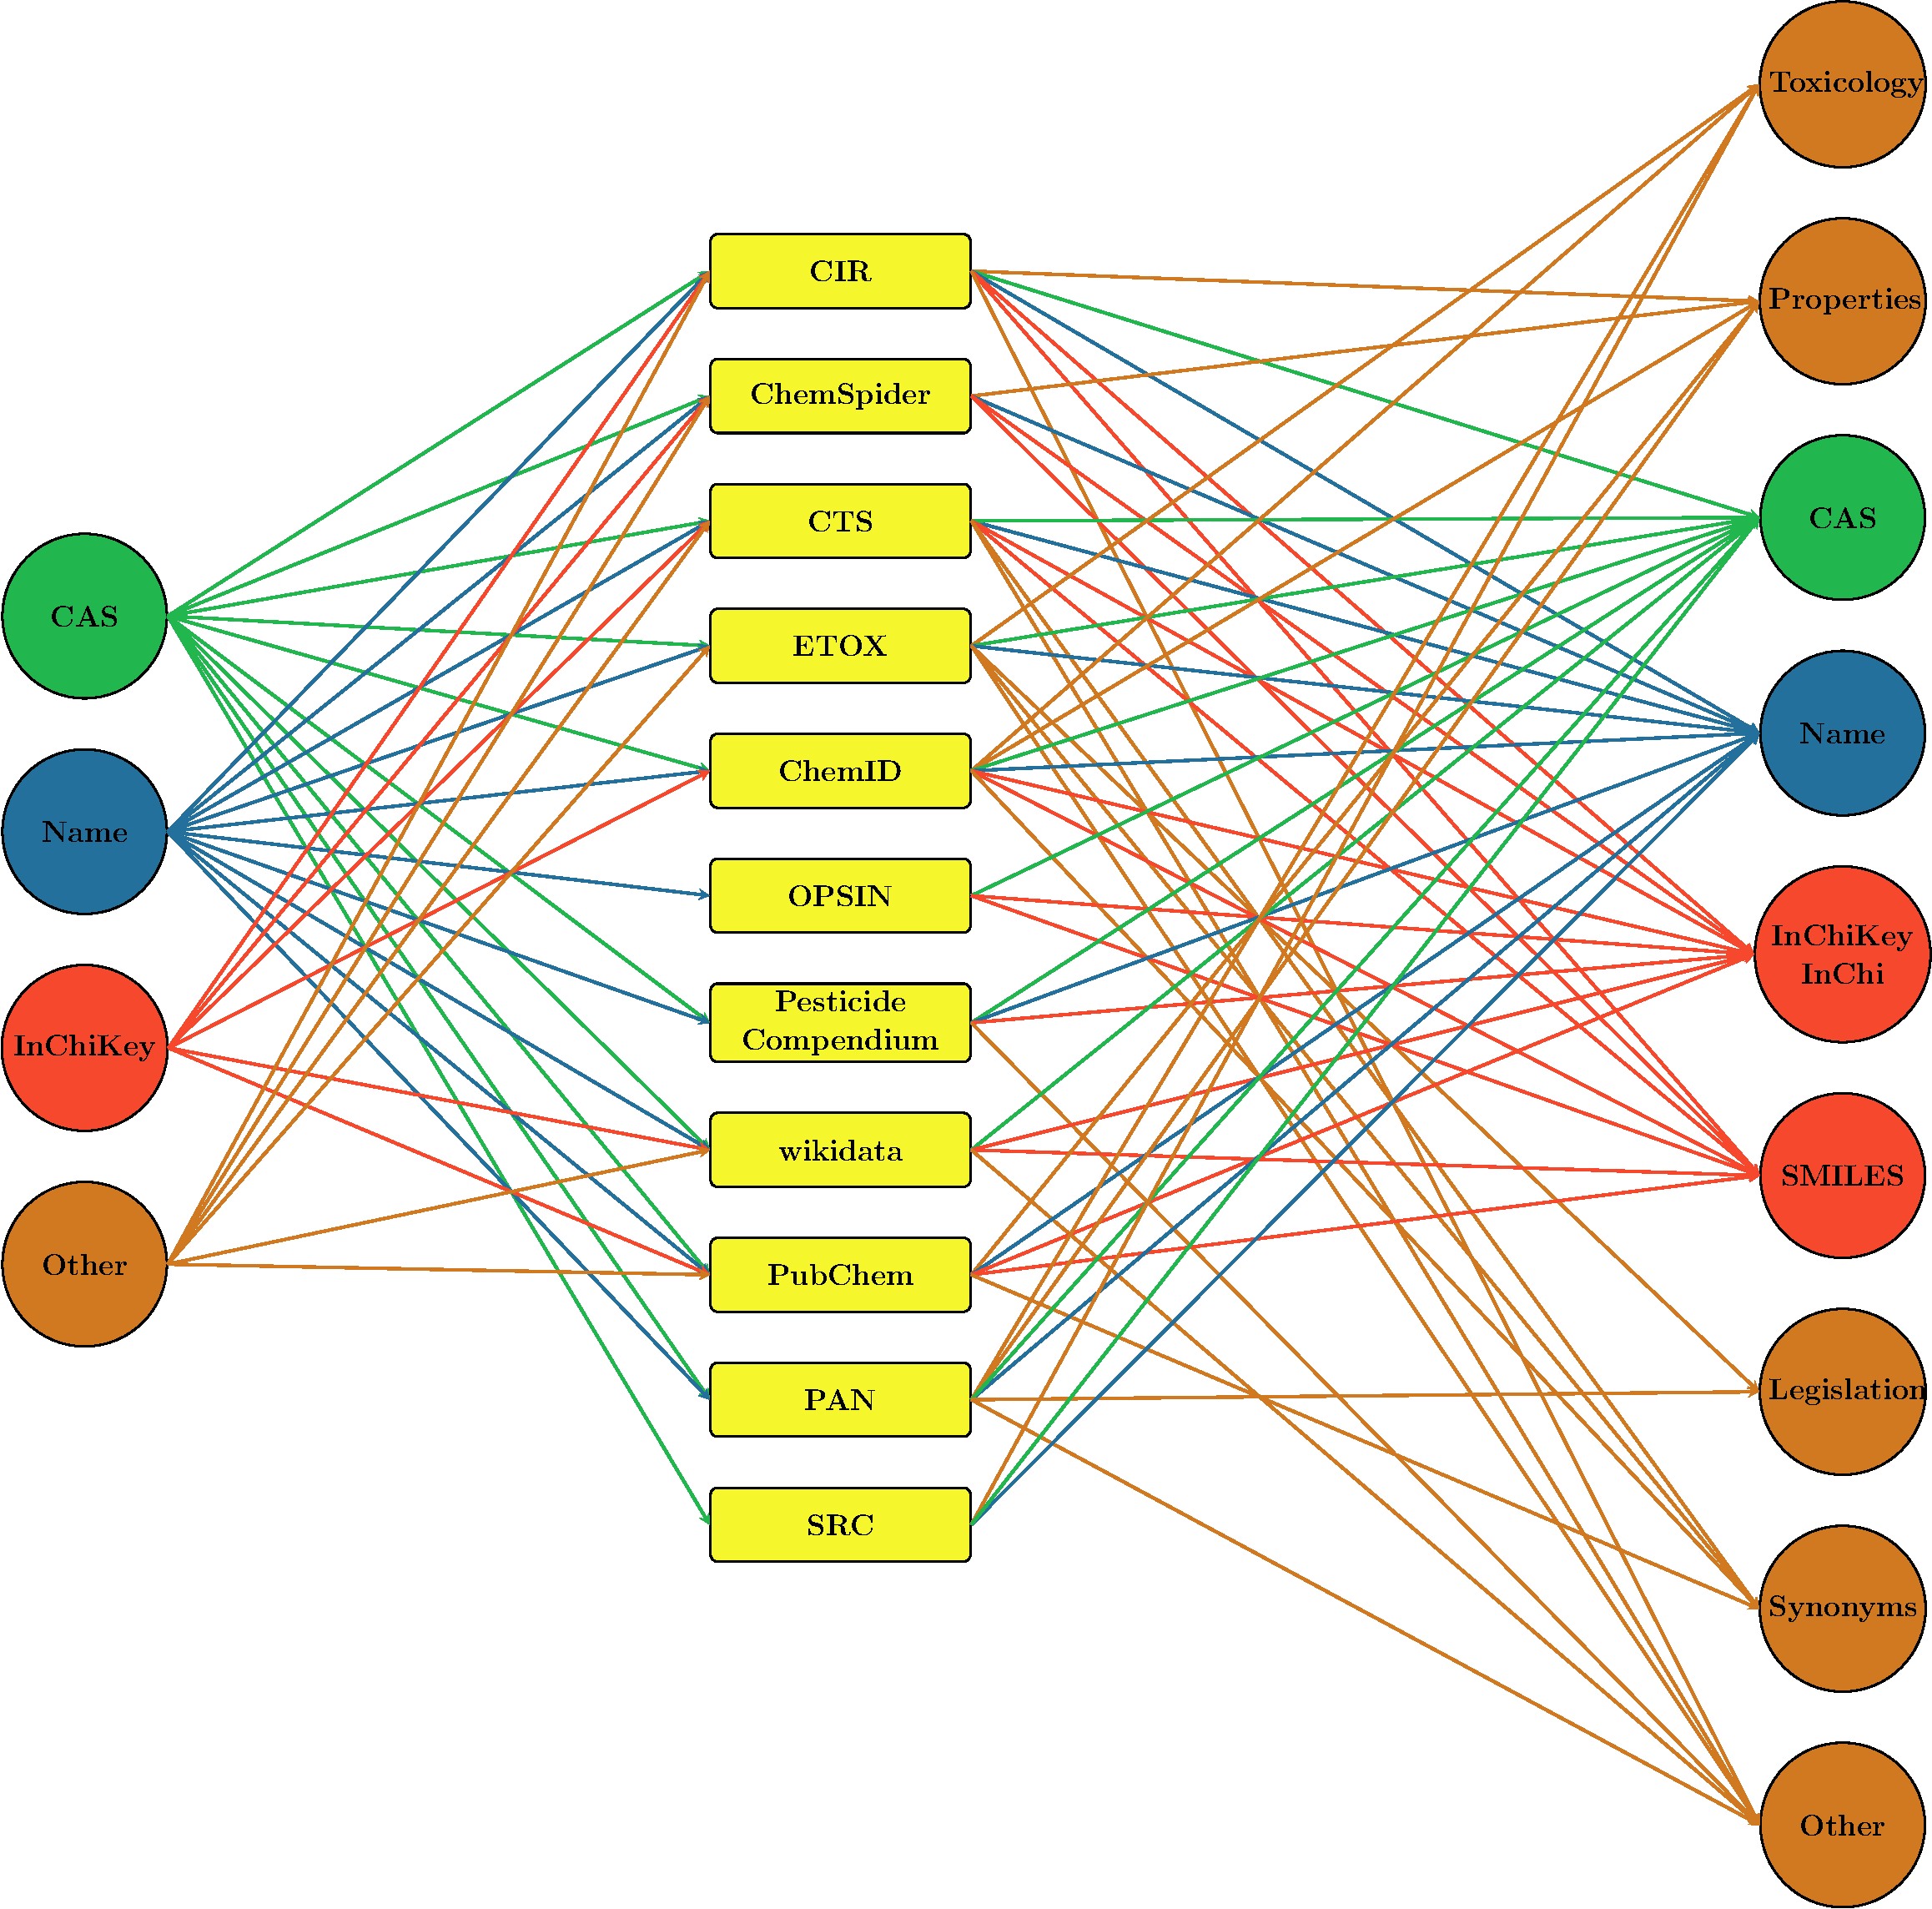
\includegraphics[width=\textwidth]{chapters/webchem/fig1.pdf}
  \caption[Overview of current data sources.]{Overview of current data sources. Input and output possibilities currently implemented in the package.}
  \label{fig:fig1}
\end{figure}


\section[Use cases]{Use cases}
\subsection[Install webchem]{Installation}
webchem can be easily installed and loaded from CRAN:

\begin{knitrout}
\color{fgcolor}\begin{kframe}
\begin{alltt}
\hlstd{R> }\hlkwd{install.packages}\hlstd{(}\hlstr{"webchem"}\hlstd{)}
\hlstd{R> }\hlkwd{library}\hlstd{(}\hlstr{"webchem"}\hlstd{)}
\end{alltt}
\end{kframe}
\end{knitrout}




The package is under active development. The latest development version is available from GitHub and also permanently available at \citet{zenodo}.
This document has been created using webchem version 0.1.


\subsection[Sample data sets]{Sample data sets}
To demonstrate the capabilities of  webchem we use two small publicly available real world data sets.
The data sets are only used for purpose of demonstration, have been slightly preprocessed (not shown) and are available through the package.

(i) jagst: This data set comprises environmental monitoring data of organic substances in the river Jagst, Germany, sampled in 2013.
The data is publicly available and can be retrieved from \citet{lubw_2016}.
It comprises concentrations  (in $\mu g~/~L$) of  34 substances  on 13 sampling occasions.
First we load the data set and inspect the first six rows:

\begin{knitrout}
\color{fgcolor}\begin{kframe}
\begin{alltt}
\hlstd{R> }\hlkwd{data}\hlstd{(}\hlstr{"jagst"}\hlstd{)}
\hlstd{R> }\hlkwd{head}\hlstd{(jagst)}
\end{alltt}
\begin{verbatim}
##         date          substance value qual
## 1 2013-01-04 2,4-Dimethylphenol 0.006    <
## 2 2013-01-29 2,4-Dimethylphenol 0.006    <
## 3 2013-02-26 2,4-Dimethylphenol 0.006    <
## 4 2013-03-26 2,4-Dimethylphenol 0.006    <
## 5 2013-04-23 2,4-Dimethylphenol 0.006    <
## 6 2013-05-22 2,4-Dimethylphenol 0.006    <
\end{verbatim}
\end{kframe}
\end{knitrout}

This data set identifies substances only by substance names. Values below the limit of quantification (LOQ) are indicated by a qualifier column.

(ii) lc50: This data consists of median acute lethal concentration for the water flea \textit{Daphnia magna} in 48 h tests ($LC_{50, D.magna, 48h}$) of 124 insecticides.
The data has been retrieved from the EPA ECOTOX database \citep{epa_2016}.

\begin{knitrout}
\color{fgcolor}\begin{kframe}
\begin{alltt}
\hlstd{R> }\hlkwd{data}\hlstd{(}\hlstr{"lc50"}\hlstd{)}
\hlstd{R> }\hlkwd{head}\hlstd{(lc50)}
\end{alltt}
\begin{verbatim}
##        cas        value
## 4  50-29-3    12.415277
## 12 52-68-6     1.282980
## 15 55-38-9    12.168138
## 18 56-23-5 35000.000000
## 21 56-38-2     1.539119
## 36 57-74-9    98.400000
\end{verbatim}
\end{kframe}
\end{knitrout}

This data set identifies the substances only by CAS numbers.


\subsection[Query identifiers]{Query identifiers}
The jagst data set covers 34 substances that are identified by (German) names.
Merging and linking these to other tables is hampered by differences and ambiguity in compound names.

One possibility to resolve this, is to use different chemical identifiers allowing easy identification.
There are several identifiers available, e.g.  registry numbers like CAS or EC, database identifiers like PubChemCID \citep{kim2016} or ChemSpiderID \citep{pence_chemspider:_2010}, line notations like SMILES \citep{Weininger_1990}, InChI and InChiKey \citep{Heller_McNaught_Pletnev_Stein_Tchekhovskoi_2015}. 
In this first example we query several identifiers to create a table that can be used as (i) supplemental information to a research article or (ii) to facilitate subsequent matching with other data.

As we are are dealing with German substance names we start to query ETOX for CAS registry numbers.
A common work flow when dealing with web resources is to 1) query a unique identifier of the source, 2) use this identifier to retrieve additional information and 3) extract the parts that are needed from the R object \citep{Chamberlain_Szocs_2013}.

First we search for ETOX internal ID numbers using the substance names:

\begin{knitrout}
\small
\color{fgcolor}\begin{kframe}
\begin{alltt}
\hlstd{R> subs} \hlkwb{<-} \hlkwd{unique}\hlstd{(jagst}\hlopt{$}\hlstd{substance)}
\hlstd{R> ids} \hlkwb{<-} \hlkwd{get_etoxid}\hlstd{(subs,} \hlkwc{match} \hlstd{=} \hlstr{'best'}\hlstd{)}
\hlstd{R> }\hlkwd{head}\hlstd{(ids)}
\end{alltt}
\begin{verbatim}
##   etoxid                           match distance                  query
## 1   8668     2,4-Dimethylphenol ( 8668 )        0     2,4-Dimethylphenol
## 2   8494 4-Chlor-2-methylphenol ( 8494 )        0 4-Chlor-2-methylphenol
## 3   <NA>                            <NA>     <NA>     4-para-nonylphenol
## 4   8397                Atrazin ( 8397 )        0                Atrazin
## 5   7240                 Benzol ( 7240 )        0                 Benzol
## 6   7331        Desethylatrazin ( 7331 )        0        Desethylatrazin
\end{verbatim}
\end{kframe}
\end{knitrout}

Only three substances could not be found in ETOX. 
Here we specify that only the \emph{`best'} match (in terms of the Levenshtein distance between query and results) is returned. 
A manual check confirms appropriate matches. 
Other options include: \emph{`all'} - returns all matches; \emph{`first'} - returns only the first match (not necessarily the best match); \emph{`ask'} - this enters an interactive mode, where the user is asked for a choice if multiple matches are found and \emph{`na'} which returns NA in case of multiple matches.

We use these data to retrieve basic information on the substances.

\begin{knitrout}
\color{fgcolor}\begin{kframe}
\begin{alltt}
\hlstd{R> etox_data} \hlkwb{<-} \hlkwd{etox_basic}\hlstd{(ids}\hlopt{$}\hlstd{etoxid)}
\end{alltt}
\end{kframe}
\end{knitrout}

webchem always returns a named list (one entry for each substance) and the available information content can be very voluminous.
Therefore, we provide extractor functions for the common identifiers: CAS, SMILES and InChIKeys.
\begin{knitrout}
\small
\color{fgcolor}\begin{kframe}
\begin{alltt}
\hlstd{R> etox_cas} \hlkwb{<-} \hlkwd{cas}\hlstd{(etox_data)}
\hlstd{R> }\hlkwd{head}\hlstd{(etox_cas)}
\end{alltt}
\begin{verbatim}
##        8668        8494        <NA>        8397        7240        7331 
##  "105-67-9" "1570-64-5"          NA "1912-24-9"   "71-43-2" "6190-65-4"
\end{verbatim}
\end{kframe}
\end{knitrout}

A variety of data are available and we cannot provide extractor functions for each of those.
Therefore, if users need to extract other data, they have to write simple extractor functions (see following examples).

In the same manner, we can now query other identifiers from another source using these CAS numbers (Figure~\ref{fig:fig1}), like PubChem


\begin{knitrout}
\begin{kframe}
\begin{alltt}
\hlstd{cids} \hlkwb{<-} \hlkwd{get_cid}\hlstd{(etox_cas)}
\hlstd{pc_data} \hlkwb{<-} \hlkwd{pc_prop}\hlstd{(cids,} \hlkwc{properties} \hlstd{=} \hlkwd{c}\hlstd{(}\hlstr{'CanonicalSMILES'}\hlstd{,} \hlstr{'InChIKey'}\hlstd{))}
\hlstd{pc_smiles} \hlkwb{<-} \hlkwd{smiles}\hlstd{(pc_data)}
\hlstd{pc_inchikey} \hlkwb{<-} \hlkwd{inchikey}\hlstd{(pc_data)}
\end{alltt}
\end{kframe}
\end{knitrout}

Finally, we combine the queried data into one data.frame

\begin{knitrout}
\begin{kframe}
\begin{alltt}
\hlstd{res} \hlkwb{<-} \hlkwd{data.frame}\hlstd{(}\hlkwc{name} \hlstd{= subs,} \hlkwc{cas} \hlstd{= etox_cas,} \hlkwc{smiles} \hlstd{= pc_smiles,}
            \hlkwc{cid} \hlstd{= pc_data}\hlopt{$}\hlstd{CID,} \hlkwc{inchikey} \hlstd{= pc_inchikey,}
            \hlkwc{stringsAsFactors} \hlstd{=} \hlnum{FALSE}\hlstd{)}
\end{alltt}
\end{kframe}
\end{knitrout}

Note that in order to use the ChemSpider functions, a personal authentication key (token) is needed, which can be retrieved from the ChemSpider web page. 
Finally, we obtain a compound table containing many different identifiers (Table~\ref{tab:comptable}), allowing easy identification and merging with other data sets, e.g.\ the lc50 data set based on CAS.

  \begin{table}[ht]
  \centering
% latex table generated in R 3.3.2 by xtable 1.8-2 package
% Fri Nov 25 18:33:30 2016
\begin{tabular}{lllll}
  \toprule
Name & CAS & SMILES & CID & InChIKey \\ 
  \midrule
2,4-Dimethylphenol & 105-67-9 & CC1=CC(... & 7771 & KUFFULV... \\ 
  4-Chlor-2-methylphenol & 1570-64-5 & CC1=C(C... & 14855 & RHPUJHQ... \\ 
  4-para-nonylphenol & - & - & - & - \\ 
  Atrazin & 1912-24-9 & CCNC1=N... & 2256 & MXWJVTO... \\ 
  Benzol & 71-43-2 & C1=CC=C... & 241 & UHOVQNZ... \\ 
  Desethylatrazin & 6190-65-4 & CC(C)NC... & 22563 & DFWFIQK... \\ 
   \bottomrule
\end{tabular}

\caption[Identifiers for the jagst data sets as queried with webchem.]{Identifiers for the jagst data sets as queried with webchem. Only the first 6 entries are shown. For SMILES and InChIKey only the first 7 characters are shown. - = not found.}
\label{tab:comptable}
\end{table}


\subsection[Toxicity of different pesticide groups]{Toxicity of different pesticide groups}
Another question we might ask is \emph{How does toxicity vary between insecticide groups?}
Answering this question would require tedious lookup of insecticide groups for each of the 124 CAS numbers in the lc50 data set.
The Compendium of Pesticide Common Names \citep{wood} contains such information and can be easily queried using CAS numbers with webchem: 

\begin{knitrout}
\begin{kframe}
\begin{alltt}
\hlstd{R> aw_data} \hlkwb{<-} \hlkwd{aw_query}\hlstd{(lc50}\hlopt{$}\hlstd{cas,} \hlkwc{type} \hlstd{=} \hlstr{'cas'}\hlstd{)}
\end{alltt}
\end{kframe}
\end{knitrout}

To extract the chemical group from the retrieved data set, we write a simple extractor function and apply this to the retrieved data:

\begin{knitrout}
\begin{kframe}
\begin{alltt}
\hlstd{igroup} \hlkwb{<-} \hlkwd{sapply}\hlstd{(aw_data,} \hlkwa{function}\hlstd{(}\hlkwc{y}\hlstd{)} \hlkwd{ifelse}\hlstd{(}\hlstr{'subactivity'} \hlopt \hlkwd{names}\hlstd{(y),}
                        \hlstd{y[[}\hlstr{'subactivity'}\hlstd{]],}
                        \hlnum{NA}\hlstd{))}
\hlstd{igroup[}\hlnum{1}\hlopt{:}\hlnum{3}\hlstd{]}
\end{alltt}
\begin{verbatim}
##                                   50-29-3 
##             "organochlorine insecticides" 
##                                   52-68-6 
##                "phosphonate insecticides" 
##                                   55-38-9 
## "phenyl organothiophosphate insecticides"
\end{verbatim}
\end{kframe}
\end{knitrout}

Figure \ref{fig:fig2} displays the result after additional data cleaning (see supplement for full code).
Overall, it took only 5 R statements to retrieve, clean and plot the data using ggplot2 \citep{ggplot2}.

\begin{figure}[ht]

\begin{knitrout}
\color{fgcolor}

{\centering 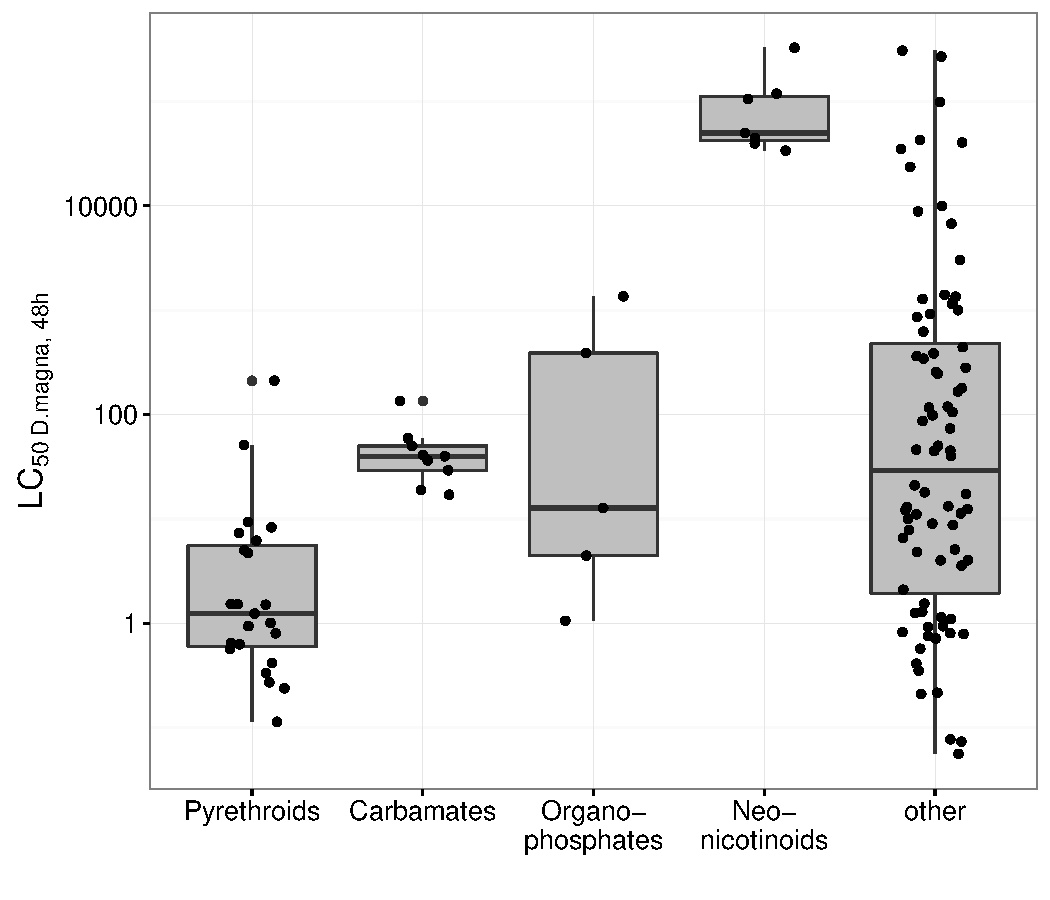
\includegraphics[width=0.7\textwidth]{chapters/webchem/plot_lc50-1.pdf}
}



\end{knitrout}
\caption[Toxicity of different pesticide groups.]{Toxicity of different pesticide groups. LC\textsubscript{50} values have been retrieved from EPA ECOTOX database, chemical groups from the Compendium of Pesticide Common Names.}
\label{fig:fig2}
\end{figure}


\subsection[Querying partitioning coefficients]{Querying partitioning coefficients}
Some data sources also provide data on chemical properties that can be queried.
Here we query for the lc50 data the $\mathrm{log}~P_{oct/wat}$ from the SRC PHYSPROP database to build a simple quantitative structure–activity relationship (QSAR) to predict toxicity.

\begin{knitrout}
\color{fgcolor}\begin{kframe}
\begin{alltt}
\hlstd{R> pp_data} \hlkwb{<-} \hlkwd{pp_query}\hlstd{(lc50}\hlopt{$}\hlstd{cas)}
\end{alltt}
\end{kframe}
\end{knitrout}

The database contains predicted and experimental values.
Extracting \\ $\mathrm{log}~P_{oct/wat}$ from the data object is slightly more complicated,  
because i) for some compounds no data could be found and ii) the data-object has a more complex structure (a data frame within a list).


\begin{knitrout}
\color{fgcolor}\begin{kframe}
\begin{alltt}
\hlstd{R> lc50}\hlopt{$}\hlstd{logp} \hlkwb{<-} \hlkwd{sapply}\hlstd{(pp_data,} \hlkwa{function}\hlstd{(}\hlkwc{y}\hlstd{) \{}
  \hlkwa{if} \hlstd{(}\hlkwd{length}\hlstd{(y)} \hlopt{==} \hlnum{1} \hlopt{&&} \hlkwd{is.na}\hlstd{(y))}
    \hlkwd{return}\hlstd{(}\hlnum{NA}\hlstd{)}
  \hlstd{y}\hlopt{$}\hlstd{prop}\hlopt{$}\hlstd{value[y}\hlopt{$}\hlstd{prop}\hlopt{$}\hlstd{variable} \hlopt{==} \hlstr{'Log P (octanol-water)'}\hlstd{]}
\hlstd{\})}
\end{alltt}
\end{kframe}
\end{knitrout}

We opted for this more complex approach, because the information available is very diverse and we cannot provide an extractor function for each purpose.
Moreover, it provides users with high flexibility regarding organisation of their data. 
Nevertheless, in the documentation of each function we provide examples on how to extract more complicated parts of the data.
The resulting data and model is displayed in Figure~\ref{fig:fig3}.

\begin{figure}[ht]
\begin{knitrout}
\color{fgcolor}

{\centering 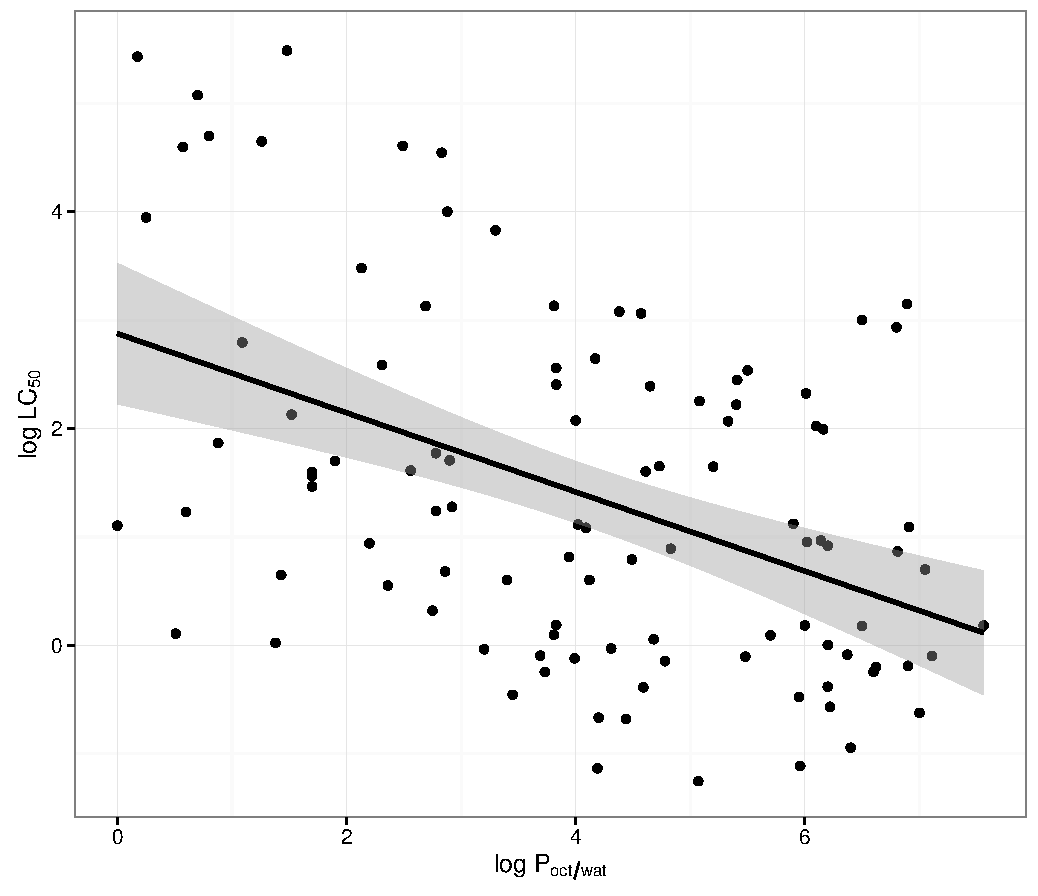
\includegraphics[width=0.7\textwidth]{chapters/webchem/plot_qsar-1.pdf} 

}



\end{knitrout}
\caption[Simple QSAR for predicting log LC\textsubscript{50} of pesticides by log P.]{Simple QSAR for predicting log LC\textsubscript{50} of pesticides by log P. 
Log P values have been retrieved from SRC Physprop database (97 experimental data, 9 estimated data and 18 substances without data). 
The line indicates the regression model ($\mathrm{log~LC}_{50} = 2.88\ensuremath{-0.37}~\mathrm{log} P$, RMSE = 1.45).}
\label{fig:fig3}
\end{figure}


\subsection[Regulatory information]{Regulatory information}
Regulatory information is of particular interest if concentrations exceed national thresholds.
In the European Union (EU) the Water Framework Directive (WFD, \citet{european_union_directive_2000}) defines Environmental Quality Standards (EQS).
Similarly, the U.S. and Canadian EPA and the WHO define Quality Standards.
Information on these standards can be queried with webchem from the PAN Pesticide Database (using pan\_query()) and from ETOX (using etox\_targets()).

In this example we search for the minimum EQS for the EU for the compounds in the jagst data set, join these with measured concentrations and evaluate wether exceedances occurred..

We re-use the above queried ETOX-IDs to obtain further information from ETOX, namely the MAC-EQS:


\begin{knitrout}
\color{fgcolor}\begin{kframe}
\begin{alltt}
\hlstd{R> eqs} \hlkwb{<-} \hlkwd{etox_targets}\hlstd{(ids}\hlopt{$}\hlstd{etoxid)}
\hlstd{R> ids}\hlopt{$}\hlstd{mac} \hlkwb{<-} \hlkwd{sapply}\hlstd{(eqs,} \hlkwa{function}\hlstd{(}\hlkwc{y}\hlstd{)\{}
  \hlkwa{if} \hlstd{(}\hlkwd{length}\hlstd{(y)} \hlopt{==} \hlnum{1} \hlopt{&&} \hlkwd{is.na}\hlstd{(y)) \{}
    \hlkwd{return}\hlstd{(}\hlnum{NA}\hlstd{)}
  \hlstd{\}} \hlkwa{else} \hlstd{\{}
    \hlstd{res} \hlkwb{<-} \hlstd{y}\hlopt{$}\hlstd{res}
    \hlkwd{min}\hlstd{(res[res}\hlopt{$}\hlstd{Country_or_Region} \hlopt{==} \hlstr{'EEC / EU'} \hlopt{&}
              \hlstd{res}\hlopt{$}\hlstd{Designation} \hlopt{==} \hlstr{'MAC-EQS'}\hlstd{,} \hlstr{'Value_Target_LR'}\hlstd{])}
  \hlstd{\}}
\hlstd{\})}
\end{alltt}
\end{kframe}
\end{knitrout}

Again, the returned information is humongous and we encourage users to study the returned objects and description of the data source.
Here, the column Designation defines the type of EQS and Value\_Target\_LR contains the value.
Unfortunately, we only found MAC-EQS values for 5 substances:

\begin{knitrout}
\color{fgcolor}\begin{kframe}
\begin{alltt}
\hlstd{R> (mac} \hlkwb{<-} \hlkwd{with}\hlstd{(ids, ids[}\hlopt{!}\hlkwd{is.na}\hlstd{(mac)} \hlopt{&} \hlkwd{is.finite}\hlstd{(mac),}
                      \hlkwd{c}\hlstd{(}\hlstr{'etoxid'}\hlstd{,} \hlstr{'query'}\hlstd{,} \hlstr{'mac'}\hlstd{)]))}
\end{alltt}
\begin{verbatim}
##    etoxid       query    mac
## 4    8397     Atrazin  2.000
## 5    7240      Benzol 50.000
## 11   8836     Irgarol  0.016
## 12   7442 Isoproturon  1.000
## 29   8756   Terbutryn  0.034
\end{verbatim}
\end{kframe}
\end{knitrout}

The get\_etoxid() function used to search ETOX-IDs returns also the original substance name (query),
so that we can easily join the table with MAC values with the measurements table :
\begin{knitrout}
\color{fgcolor}\begin{kframe}
\begin{alltt}
\hlstd{R> jagst_eqs} \hlkwb{<-} \hlkwd{merge}\hlstd{(jagst, mac,} \hlkwc{by.x} \hlstd{=} \hlstr{'substance'}\hlstd{,} \hlkwc{by.y} \hlstd{=} \hlstr{'query'}\hlstd{)}
\hlstd{R> }\hlkwd{head}\hlstd{(jagst_eqs)}
\end{alltt}
\begin{verbatim}
##   substance       date  value qual etoxid mac
## 1   Atrazin 2013-09-10 0.0068    =   8397   2
## 2   Atrazin 2013-10-08 0.0072    =   8397   2
## 3   Atrazin 2013-03-26 0.0040    =   8397   2
## 4   Atrazin 2013-04-23 0.0048    =   8397   2
## 5   Atrazin 2013-11-05 0.0036    =   8397   2
## 6   Atrazin 2013-07-16 0.0052    =   8397   2
\end{verbatim}
\end{kframe}
\end{knitrout}

Finally, we can compare the measured value to the MAC, which reveals that there have been no exceedances of these 5 compounds.




\subsection[Utility functions]{Utility functions}
Furthermore, webchem provides also basic functions to check identifiers that can be used for data quality assessment.
The functions either use simple formatting rules,

\begin{knitrout}
\color{fgcolor}\begin{kframe}
\begin{alltt}
\hlstd{R> }\hlkwd{is.inchikey}\hlstd{(}\hlstr{'BQJCRHHNABKAKU-KBQPJGBKS-AN'}\hlstd{)}
\end{alltt}


{\ttfamily\noindent\itshape\color{messagecolor}{\#\# Hyphens not at position 15 and 26.}}\begin{verbatim}
## [1] FALSE
\end{verbatim}
\begin{alltt}
\hlstd{R> }\hlkwd{is.cas}\hlstd{(}\hlstr{'64-17-6'}\hlstd{)}
\end{alltt}


{\ttfamily\noindent\itshape\color{messagecolor}{\#\# Checksum is not correct! 5 vs. 6}}\begin{verbatim}
## [1] FALSE
\end{verbatim}
\end{kframe}
\end{knitrout}

or web resources like ChemSpider
\begin{knitrout}
\color{fgcolor}\begin{kframe}
\begin{alltt}
\hlstd{R> }\hlkwd{is.inchikey}\hlstd{(}\hlstr{'BQJCRHHNABKAKU-KBQPJGBKSA-5'}\hlstd{,}
  \hlkwc{type} \hlstd{=} \hlstr{'chemspider'}\hlstd{)}
\end{alltt}
\begin{verbatim}
## [1] FALSE
\end{verbatim}
\end{kframe}
\end{knitrout}


\clearpage
\section[Discussion]{Discussion}
\subsection[Related software]{Related software}
Within the R ecosystem, there are only a few similar projects:
rpubchem \citep{rpubchem_2014} provides an interface to PubChem.
Similarly, ChemmineR \citep{chemminer_2008}, a mature chemo-informatics package, provides an interface to Pubchem. 
webchem does not provide any chemo-informatic functionality, but integrates access to many data sources.
WikidataR \citep{wikidatar_2016} provides an interface to wikidata that could be used to retrieve chemical data from Wikipedia.
However, it does not provide predefined methods for chemical data like webchem.
Within the Python ecosystem the libraries PubChempy \citep{pubchempy}, ChemSpiPy \citep{chemspipy} and CIRpy \citep{cirpy} are available for similar tasks as those outlined here.
webchem is not specialized and tries to integrate many data sources and for some of these it provides a unique programmatic interface.
The Chemical Translation Service \citep{wohlgemuth_haldiya_willighagen_kind_fiehn_2010}, which is also one of the sources that can be queried, allows batch conversion of chemical identifiers.
However, it does not provide access to other data (experimental, modeled or regulatory data).


\subsection[Open Science]{Open Science}
An increasing number of scientific data is becoming publicly available \citep{Gewin_2016, Reichman_Jones_Schildhauer_2011,Boyle_Guha_2011}, either in public data repositories or as supplement to publications.
To be usable for other researchers chemical compounds should be properly identified, not only by chemical names but also with accompanying identifiers like InChIKey, SMILES and authority-assigned identifiers.
webchem provides an easy way to create such meta tables as shown in Table \ref{tab:comptable} and facilitates chemical data availability to researchers.
However, good quality of data is crucial for every analysis \citep{stieger2014} and additional effort and methods are needed to validate data quality.

\subsection[Further development]{Further development}
We have outlined only a few use cases that will likely be useful for many researchers.
Given the huge amount of publicly available information, many other possibilities can be envisioned.
webchem is currently under active development and several other data sources have not been implemented yet but may be in the future.
GitHub makes contributing easy and we strongly encourage contribution to the package.
Moreover, comments, feedback and feature requests are highly welcome.


\section[Conclusions]{Conclusions}
Researchers need to have easy access to global knowledge on chemicals.
webchem can save \emph{"hundreds of working hours"} gathering this knowledge \citep{munchalizia2016}, so that researchers can focus on other tasks.



%% ----------------------------------------------------------------------------
\clearpage
\section{References}
\printbibliography[heading=none]
